%=========== Custom Commands =============
% Roman numerals
\makeatletter
\newcommand*{\rom}[1]{\Ifstr{#1}{0}{0}{\expandafter\@slowromancap\romannumeral #1@}}
\makeatother

% Text for writing the edition
\newcommand*{\editiontext}{
    \editionnumber~Edition~\Ifstr{\buildnumber}{}{}{(Build \buildnumber)}
}

%============= Front Matter ==============
\Ifstr{\isebook}{true}{
    % Title page
    \begin{titlepage}
        \newgeometry{hmargin=2cm, vmargin=2.5cm}

        \AddToShipoutPictureBG*{%
            \AtPageLowerLeft{%
                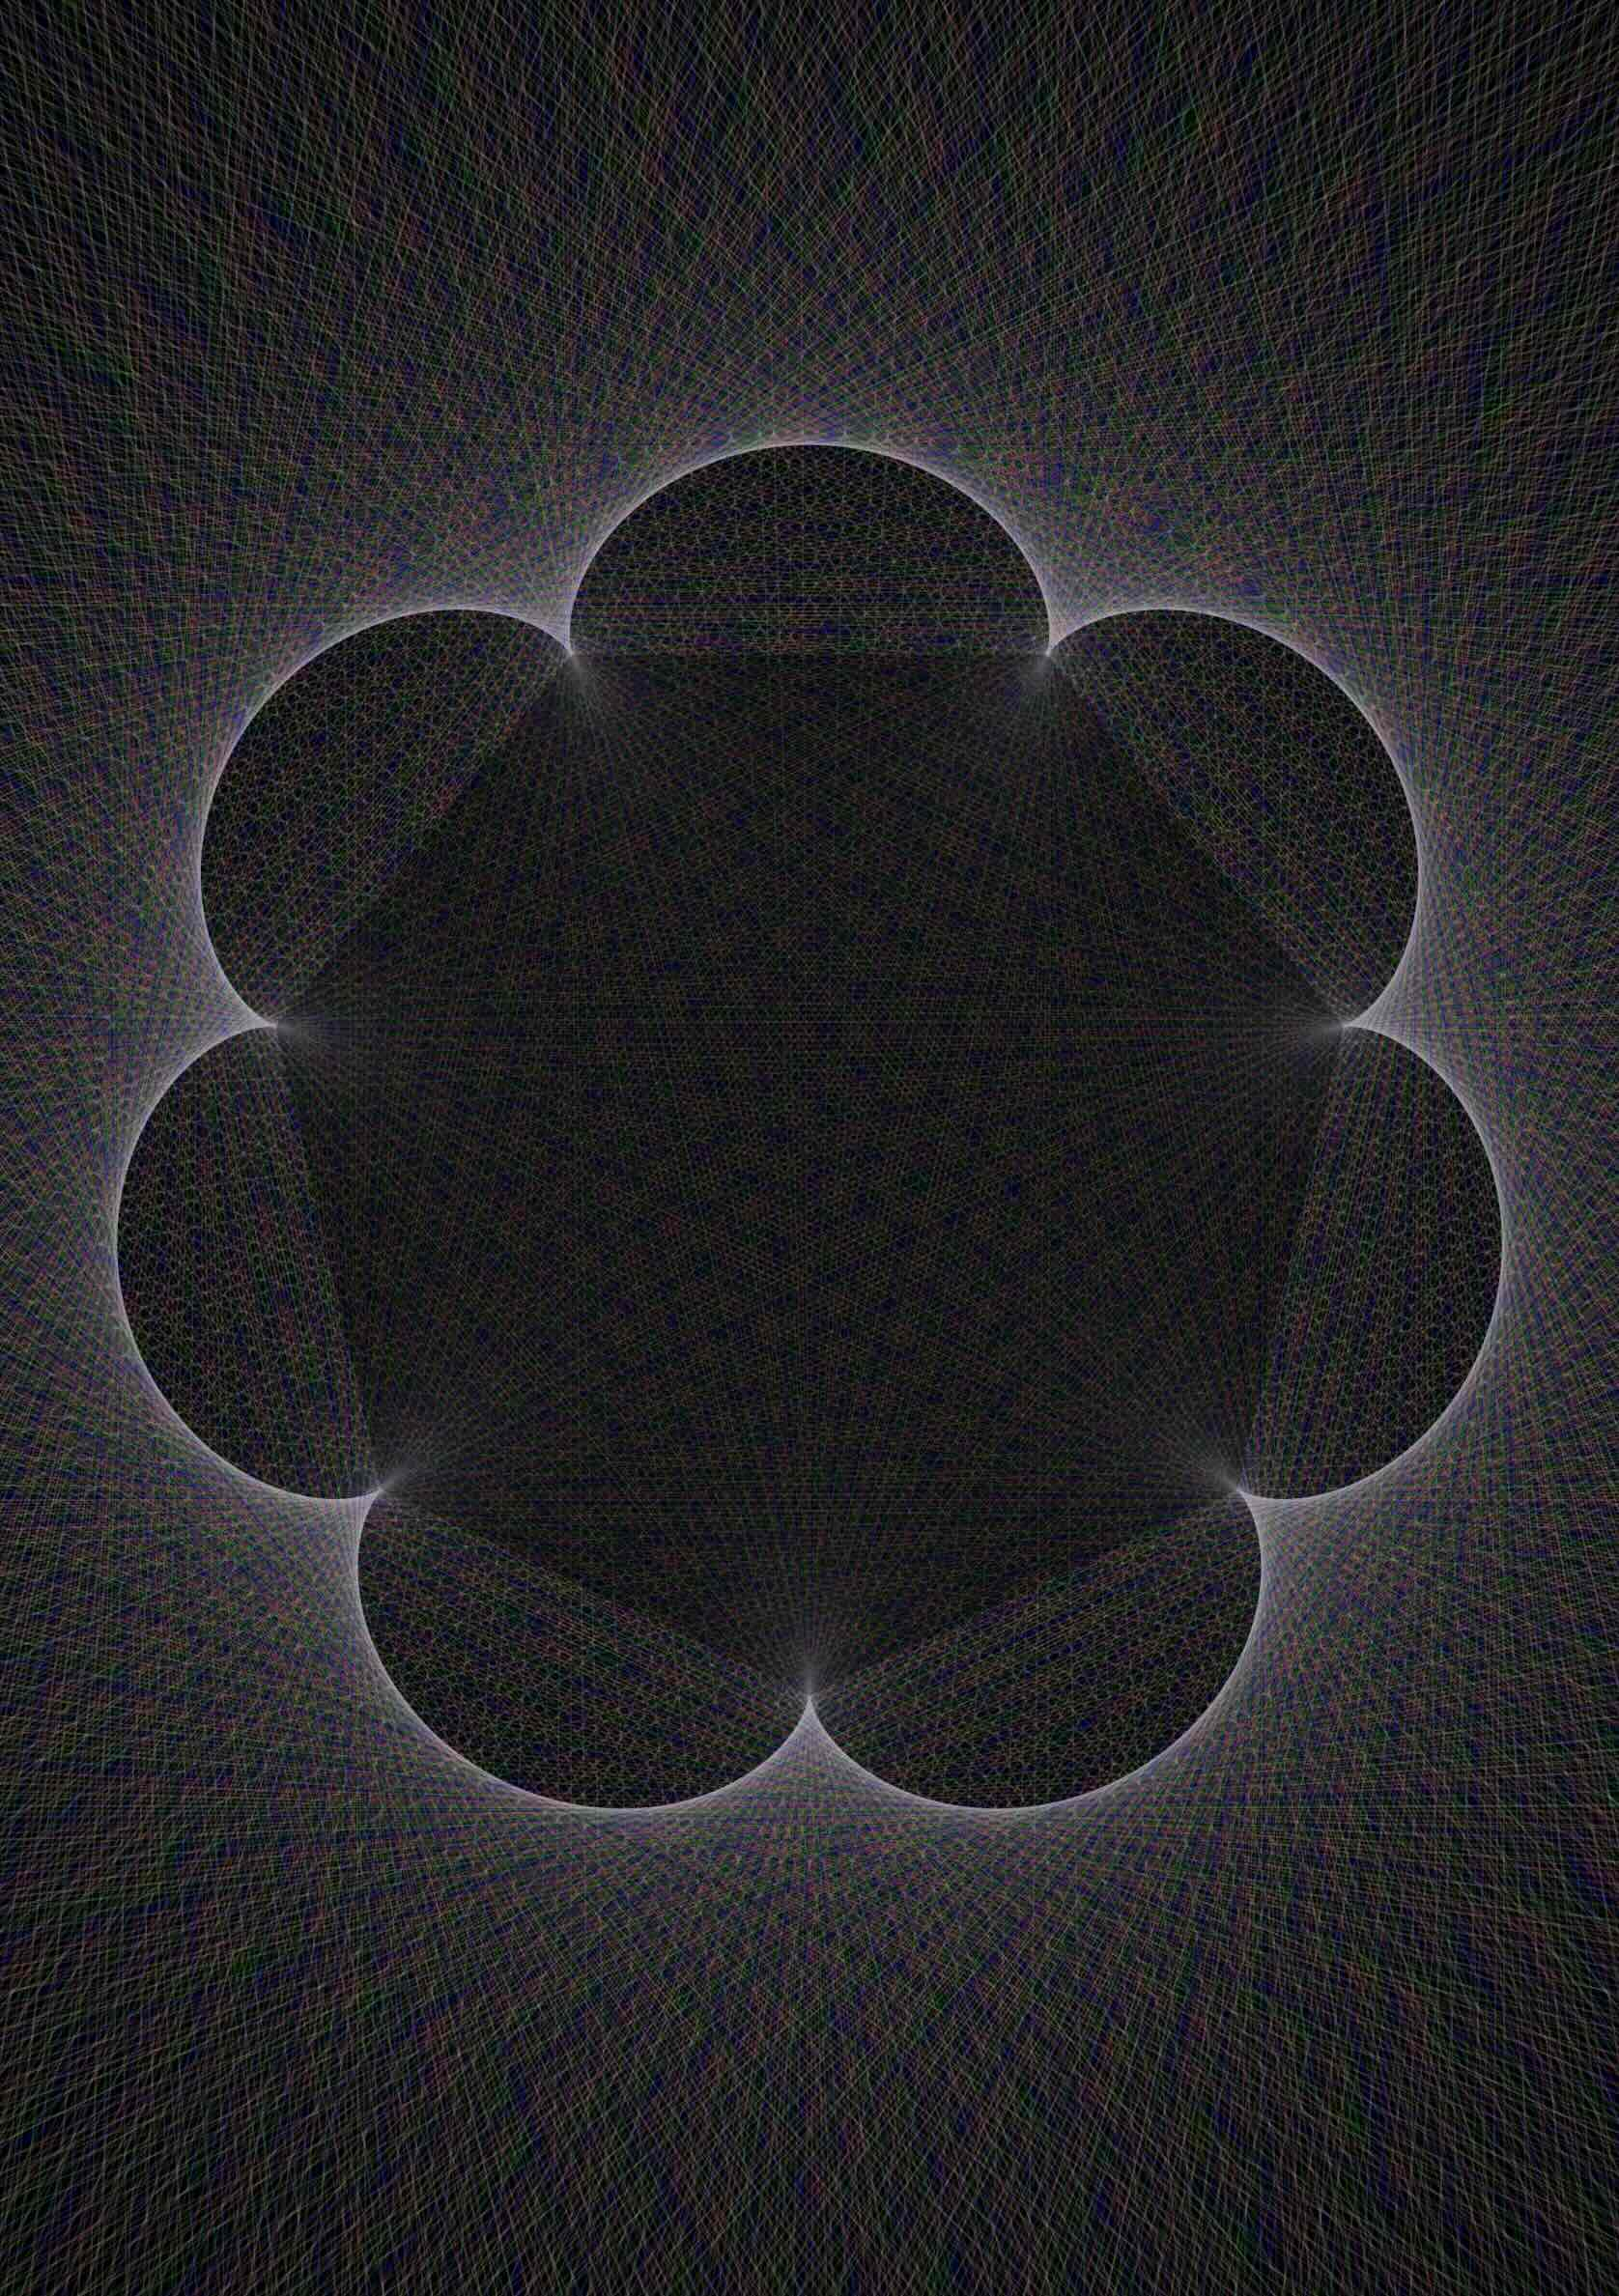
\includegraphics[width=\paperwidth,height=\paperheight]{images/cover/cover-page-background.jpg}%
            }%
        }

        \vspace*{\fill}
        \vspace{0.4cm}  % To make "ABSTRACT ALGEBRA" centred

        \begin{center}
            \color{white}

            {\fontsize{18pt}{0pt}\selectfont \textbf{A Complete}\\\textbf{Introduction to}}\\

            \vspace{0.4cm}
            {\fontsize{44pt}{0pt}\selectfont \textbf{ABSTRACT}}\\
            \vspace{0.15cm}
            {\fontsize{44pt}{0pt}\selectfont \textbf{ALGEBRA}}\\

            \vspace{0.5cm}
            {\fontsize{14pt}{0pt}\selectfont \editiontext}\\

            \vspace{1.25cm}
            {\fontsize{20pt}{0pt}\selectfont Kan Onn Kit}\\
        \end{center}
        \vspace*{\fill}
    \end{titlepage}
}{
    % Half title page
    \thispagestyle{empty}
    \null\vspace{4cm}
    \begin{raggedleft}
        {\fontsize{24pt}{0pt}\selectfont \textbf{A Complete Introduction to Abstract Algebra}}\\
    \end{raggedleft}

    % Title page
    \begin{titlepage}
        \null\vspace{4cm}
        \begin{raggedleft}
            {\fontsize{20pt}{0pt}\selectfont \textbf{A Complete}\\\textbf{Introduction to}}\\

            \vspace{0.4cm}
            {\fontsize{48pt}{0pt}\selectfont \textbf{ABSTRACT}}\\
            \vspace{0.15cm}
            {\fontsize{48pt}{0pt}\selectfont \textbf{ALGEBRA}}\\

            \vspace{0.5cm}
            {\fontsize{16pt}{0pt}\selectfont \editiontext}\\

            \vspace{1.25cm}
            {\fontsize{20pt}{0pt}\selectfont Kan Onn Kit}\\
        \end{raggedleft}
        \vspace*{\fill}
    \end{titlepage}
}

\newpage{}

% Edition notice
\clearpage\null\vfill
\thispagestyle{empty}
\begin{minipage}[b]{0.9\textwidth}
    \footnotesize\raggedright
    \setlength{\parskip}{0.5\baselineskip}

    Published by Kan Onn Kit\\
    Singapore
    \vspace{5cm}

    \textbf{A Complete Introduction to Abstract Algebra}\par
    \editiontext
    \vspace{0.3cm}

    Copyright \copyright \ 2022 -- \the\year\ Kan Onn Kit\par
    This work is licensed under a Creative Commons Attribution-ShareAlike 4.0 International Licence.\par
    \pdfteximg{2.5cm}{images/CC_BY-SA_4.0.pdf_tex}\\
    The full licence text is available at \url{http://creativecommons.org/licenses/by-sa/4.0/}.\par
    The source files for this book are available at \url{https://github.com/PhotonicGluon/Abstract-Algebra-Book}.
    \vspace{0.3cm}

    Typeset in 10pt \TeX~Gyre Pagella using PDF\LaTeX.
\end{minipage}

\vspace*{2\baselineskip}
\cleardoublepage

% Dedication page
\thispagestyle{empty}
\vspace*{1cm}

\begin{center}
    {\fontsize{18pt}{0}\selectfont \textit{For my friends}}\\
\end{center}

\vspace*{1.5cm}

\begin{center}
    \parbox{10cm}{
        \Large
        Symmetry is a vast subject, significant in art and nature. Mathematics lies at its root, and it would be hard to find a better one on which to demonstrate the working of the mathematical intellect.
        \vspace{0.3cm}

        \hfill
        --- Hermann Weyl, 1952\\
        \vspace{-0.7cm}

        \hfill
        \normalsize
        ({\cite[p.~145]{weyl_1952}})
    }
\end{center}

\vspace*{\fill}

% "Content for no one... where you hide something so deeply that you don't care if anyone finds it [because] you just like knowing that it's there"
\begin{center}
    \fontsize{8pt}{8pt}\selectfont
    \code{3402 0604 1805 0000 0606 2802 1005 0000 1101 0102 0000 2201 1109 2003\\0202 1504 0000 0608 0107 0502 1111 2705 0000 1002 1701 2901 2301 2602}
\end{center}

\vspace*{2\baselineskip}
\cleardoublepage

% Table of contents
\createtoc

% Errata
\chapter{Errata}
Mathematics is unforgiving in its level of rigour and precision in its results; errors are the antithesis of this. When writing this book, I strove for accuracy, clarity, and precision in the terms used in the book and the results presented therein. I wanted to ensure that this book explained all concepts thoroughly and in a way accessible for someone who started with no knowledge of abstract algebra. However, despite numerous revisions, it is unfortunate that some errors may slip unnoticed. I deeply regret any inconvenience that these errors have caused.

A list of corrections are available on the GitHub repository containing the source code of this book. The list will be updated whenever a new error is spotted, or if a clarification needs to be made. You can find this list at \url{https://github.com/PhotonicGluon/Abstract-Algebra-Book/blob/main/errata/errata.pdf}. In addition, if you find any more errors in the book, please report them at \url{https://github.com/PhotonicGluon/Abstract-Algebra-Book/issues}.

% Acknowledgements
\chapter{Acknowledgements}
Undertaking such a monumental project is new to me, and I am indebted to the people who accompanied me on this journey.

I am eternally grateful to my parents, who have spent countless hours and an ungodly amount of effort to raise me into who I am today. Their omnipresent kindness, patience, and love for me are something I certainly do not deserve, and I cannot thank them enough for taking care of me throughout our highs and lows.

I would like to thank my tutor, Leong Chong Ming, for getting me interested in abstract algebra in the first place. His enthusiasm and eagerness to share his knowledge on the subject are the driving forces behind my writing this book.

I am grateful for the help of my friend Low Ji Yuan, who has assisted me with countless revisions of this book's content and given me another pair of eyes to vet it. Without her, many errors would have gone unnoticed.

My utmost appreciation, gratitude, and thanks go to Joshua Foo Yong Yi, who also helped proofread countless drafts of this book since its inception. He has also personally sat through lessons about abstract algebra with me using this book, allowing me to fix countless errors I would not have otherwise spotted. I cannot thank him enough.

I also sincerely appreciate the continued support from my mathematics tutors, Loke Weng Heng, Siow Yun Jie, and Teng Yen Ping. They have been there through my junior college years, inspiring me with the wonders of mathematics. I am indebted to them for allowing me to excel in my final examinations.

My close friends, Aidan Tay, Gabriel Fong, and Low Ji Yuan, have accompanied me through two years of schooling (and maths jokes). I offer infinite thanks to them for sticking with me and encouraging this maths nerd to pursue his wacky projects.

A thousand thanks go out to my teachers at the School of Science and Technology, Singapore, and specifically to my form teacher, Lee Tsi Yew Samuel, who instilled important character values in me so that I can excel in my future endeavours.

Last but not least, thank you for picking up this book.

% Preface
\chapter{Preface}
Although algebra has a long history, it has undergone striking changes in the past few decades. Many recognise abstract algebra as an essential element of higher mathematical education. However, its results are often hard to grasp and understand without prerequisite knowledge or a heavy background in mathematics. Most books on this subject are crafted for undergraduates at universities. They are not for a general mathematics enthusiast or one who seeks to understand more about the inner structure of algebra that mathematicians encounter frequently.

Exploration of such structures is fundamental to the current underpinning of scientific inquiries. For example, groups are important as they describe the symmetries that the laws of physics seem to obey. Finite fields are also used in coding theory and combinatorics. I hope this book will inspire more people to learn more about abstract algebra beyond the simple introduction presented here.

In addition, in most textbooks, essential details are left for the reader to figure out independently without providing additional guidance or help. Numerous textbooks provide exercises and problems for the different topics taught in abstract algebra. Still, only a few written solutions are provided for the questions and problems posed, leaving readers unsure of the correctness of their answers. The completeness of a textbook is essential; no claim made should be without justification (unless necessary). This book offers a complete picture of abstract algebra by providing full-worked solutions to all exercises and problems.

This book achieves several goals. First, it adequately explains the core results from abstract algebra without assuming any sophisticated prior knowledge, such as number theory or modular arithmetic. This book can serve as a self-contained reference to anyone looking to pick up abstract algebra out of interest. I hope anyone who wishes to do so does not have to look up any information online to supplement missing details.

In addition, this book can demystify the core steps many textbooks gloss over when providing significant results or when writing solutions to problems and exercises. In those textbooks, the reader is expected to fill in the missing details, and possible errors that could be committed when attempting to complete solutions may go unnoticed without guidance. By providing written solutions to the results, this book would hopefully alleviate any issues with determining the correctness of one's solution to exercises and problems posed.

Finally, I hope this book can make the results of this wondrous field as accessible, approachable, and understandable as possible. The field of abstract algebra, although not immediately apparent, underpins most discussions of mathematics today, and one cannot escape from its influence in its entirety. Therefore, a thorough understanding of the basics of such a fundamental subject must be conveyed appropriately, lest we risk this beautiful field being resigned to exclusivity by those who can understand it.

In closing, I recall two famous quotes from two mathematicians. The first by Godfrey Harold Hardy:
\quoteattr[0.5cm]{
    \normalshape
    We have concluded that the trivial mathematics is, on the whole, useful, and that the real mathematics, on the whole, is not.
    }
    {G.H. Hardy}
    {\cite[p.~43]{hardy_snow_1969}}

The second by Paul Lockheart:
\quoteattr[0.5cm]{
    \normalshape
    Mathematics is \textit{the music of reason}. To do mathematics is to engage in an act of discovery and conjecture, intuition and inspiration; to be in a state of confusion -- not because it makes no sense to you, but because you gave it sense and you still don't understand what your creation is up to; to have a breakthrough idea; to be frustrated as an artist; to be awed and overwhelmed by an almost painful beauty; to be \textit{alive}, damn it.
    }
    {Paul Lockheart}
    {\cite[p.~8]{lockheart_2002}, emphasis his}

I hope this book can accomplish these goals and let readers enjoy the wonders of abstract algebra.
\hfill{\textit{3 August, 2024}}

% Suggestions on the use of this book
\chapter{Suggestions on the Use of This Book}
\section*{General Information}
\begin{itemize}
    \item This book includes two types of questions for readers: exercises and problems. For most chapters, we include both.
    \begin{itemize}
        \item An exercise can be thought of as a ``self-review'' question. Exercises ensure that the content of a particular section is understood and relatively simple to answer.
        \item A problem is a more holistic version of an exercise. Generally, solutions to problems require a thorough understanding of the current chapter.
    \end{itemize}
    We include full solutions to both exercises and problems. Note that these are just suggested answers; other approaches may be valid.

    \item Results and questions have differing numbering systems.
    \begin{itemize}
        \item All definitions, axioms, examples, lemmas, theorems, propositions, and corollaries are consecutively numbered using the format
        \begin{quote}
            \code{[CHAPTER].[SECTION].[NUMBER]}
        \end{quote}
        For example, the fourth statement in chapter 2, section 3, is labelled \textbf{2.3.4}.
        \item Exercises and problems are also numbered consecutively using the format
        \begin{quote}
            \code{[CHAPTER].[NUMBER]}
        \end{quote}
        For example, the third exercise in chapter 2 is labelled \textbf{2.3}. Likewise, the fourth problem in chapter 3 is labelled \textbf{3.4}.
    \end{itemize}
    \item For more technical proofs, we include a sketch of the proof along with the full proof. The symbol ``$\qedsketch$'' marks the end of the sketch of a proof, while ``$\qedproof$'' marks the end of a proof.
\end{itemize}

\section*{Chapter Interdependence}
The diagram on the next page shows chapter interdependence. It should be used in conjunction with the table of contents and notes listed.

\newpage
\begin{center}
    \pdfteximg{\linewidth}{images/interdependence.pdf_tex}
\end{center}

\newpage

\textbf{Notes}:
\begin{itemize}
    \item Part 0 is required reading for future parts of the book. Readers who are already familiar with the content in part 0 can proceed directly to part I.
    \item Part I on groups is the fundamentals of abstract algebra.
    \begin{itemize}
        \item Chapter 7 is essentially independent from the rest of the other chapters. It provides motivation for the axioms of groups, but readers who want to skip this introduction can move straight to chapter 9.
        \item Chapters 8, 9, and 10 are the essentials of group theory.
        \item Chapter 10 is required reading for chapters 11, 12, 13, and 15.
        \item Chapter 13 only requires knowledge of the subgroup product from chapter 12 (specifically \myref{definition-subgroup-product} and \myref{prop-subgroup-product-is-subgroup}); otherwise these two chapters are relatively independent.
        \item Chapter 14 assumes knowledge of chapter 13, and knowledge of permutations and the symmetric group from chapter 11.
        \item Usually, group actions (chapter 15) would be read after the essentials of group theory; therefore chapter 15 could be read after chapter 10.
        \item Chapter 16 only requires chapters 13 and 15.
        \item Chapter 17 on the requires knowledge about direct products (chapter 12) and the Sylow Theorems (chapter 16). Knowledge about cyclic groups (\myref{section-more-about-cyclic-groups}) is the only content required from chapter 14.
        \item Chapter 18 only require results from chapter 13, except for \myref{problem-S4-composition-series} which uses the alternating group introduced in chapter 14.
        \item Chapter 19 assumes full knowledge of chapter 13; minor results from chapter 14 (specifically, results about the alternating group), chapter 16 (the Third Sylow Theorem, \myref{thrm-sylow-3}), and chapter 18 (\myref{problem-S4-composition-series}) are required.
    \end{itemize}
    \item Part II on rings builds on ideas from part I.
    \begin{itemize}
        \item Before starting on chapter 20, on the introduction to rings, it is recommended to read chapters 8, 9, 10, 13, and 14 from group theory. This way, a firm foundation of the terminology used in chapter 20 onwards would be built. However, not all content from chapter 14 is relevant for ring theory. The critical sections are \myref{section-more-about-cyclic-groups}, \myref{section-group-of-units-mod-n}, and \myref{section-groups-of-matrices}.
        \item Chapter 23 could be read after chapter 21; only \myref{section-prime-and-maximal-ideals} on prime and maximal ideals and \myref{problem-non-trivial-prime-ideal-is-maximal-in-PID} requires knowledge from chapter 22.
        \item Chapter 24 requires chapter 22, but mostly does not require chapter 22; only \myref{problem-integral-domain-iff-trivial-ideal-is-prime} requires knowledge of chapter 22 and knowledge of \myref{section-prime-and-maximal-ideals}, which requires chapter 22 as well.
        \item Chapter 25 assumes knowledge of chapter 24, and requires the whole of chapter 22.
        \item Chapter 26 requires chapter 25.
        \item Chapter 28 can be read after chapter 25, since it only requires familiarity with polynomial rings. The content of chapter 28 is relatively independent from the rest of ring theory, so readers may also choose to skip it.
    \end{itemize}
    \item Part III on fields builds upon the results of rings in part II, which should naturally occur since fields are rings but with more properties.
    \begin{itemize}
        \item Chapter 29 on the basics of fields assumes knowledge from most chapters from ring theory except chapter 28. It also requires knowledge from chapter 15 (group actions), especially Cauchy's theorem (\myref{thrm-cauchy}).
        \item Chapter 33 on finite fields requires knowledge of the Fundamental Theorem of Finite Abelian Groups (\myref{thrm-fundamental-theorem-of-finite-abelian-groups}) as it is used to describe the structure of finite fields.
    \end{itemize}
    \item Part IV on Galois theory is the final part of the book, providing a connection between field theory and group theory.
    \begin{itemize}
        \item Chapter 35 on Galois theory requires the results from all the previous chapters, except for chapter 28 (the NTRU cryptosystem).
        \item Chapter 36, the final chapter, is on the Fundamental Theorem of Algebra. It provides a conclusion to all the content covered in these books, wrapping up the exploration of Galois theory and introduces some elementary real analysis concepts.
    \end{itemize}
\end{itemize}
